%!TEX root = ../main.tex

\section{Local Storage}
Somewhere this should be answered!

How should local data storage be realised?

\section{Software on Stationary Computer}
The stationary computer needs to receive data through wifi and decode the received messages using the protocol that is to be developed.
A user should be able to access the data through an API.
This API should act as the front-end of the underlying network.
As a proof of concept, a simple UI should be implemented to show how data can be presented to the user.
The software also needs the ability to let the user send a command to the on-vehicle network to start and stop specific nodes.
As with the previous parts of the system, this program should be compatible with linux.
The described software is outlined in figure \ref{fig:setup_ui}.

\begin{figure}[h]
	\centering
	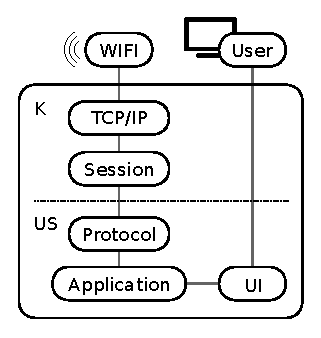
\includegraphics{graphics/stationary_software.eps}
	\caption{Structure of software on stationary computer.}
	\label{fig:setup_ui}
\end{figure}

\subsection{Protocol}
As described in section \ref{sec:canbusanalysis}, a custom protocol will be developed to complement CAN.
Any data received through the WiFi will be encoded using this protocol.
It is the responibility of this software to decode the software in order to present it to the user in a readable format.
In order to maintain the modularity of the system, the decoding should be done in such a way that future developers can easily add new nodes, and with them, new decoding for data types.

\subsection{Application}
The system is intended to function as a monitoring system of go-kart data.
Presentation of the data is not the focus of the project and as such only a rudimentary UI is developed to show the functionality.
The software should however be designed in such a way that a developer can easily create a custom (G)UI for the system, which fits the needs of that particular project.
In order to create the most seamless interface for this functionality the software should implement an API which acts as a front-end for the underlying network.
The API-approach has the added benefit of allowing the user to use the incoming data in any way that may suit their project.
